%  This is a LaTex file.

%  Homework for the course "AMath 585:  Applied Linear Algebra and Numerical Analysis", 
%  Autumn quarter, 2009, Anne Greenbaum.


%   A latex format for making homework assignments.


\documentclass[letterpaper,12pt]{article}

%          The page format, somewhat wider and taller page than in art12.sty.

\topmargin -0.1in \headsep 0in \textheight 8.9in \footskip 0.6in
\oddsidemargin 0in  \evensidemargin 0in  \textwidth 6.5in
\usepackage{graphicx}
\usepackage{listings}
\usepackage{caption}
\usepackage{subcaption}
\usepackage{color}
\usepackage{float}
\definecolor{keywords}{RGB}{255,0,90}
\definecolor{comments}{RGB}{0,0,113}
\definecolor{red}{RGB}{160,0,0}
\definecolor{green}{RGB}{0,150,0}
\definecolor{codegreen}{rgb}{0,0.6,0}
\definecolor{codegray}{rgb}{0.5,0.5,0.5}
\definecolor{codepurple}{rgb}{0.58,0,0.82}
\definecolor{backcolour}{rgb}{0.95,0.95,0.92}
\definecolor{brown}{rgb}{0.59, 0.29, 0.0}
\definecolor{beaublue}{rgb}{0.74, 0.83, 0.9}
\definecolor{orange}{rgb}{1.0, 0.5, 0.0}
\definecolor{darkslategray}{rgb}{0.18, 0.31, 0.31}
\definecolor{deepblue}{rgb}{0,0,0.5}
\definecolor{deepred}{rgb}{0.6,0,0}
\definecolor{deepgreen}{rgb}{0,0.5,0}
\lstdefinestyle{myMatlabstyle}{
	language=Matlab,
	backgroundcolor=\color{white},   
	commentstyle=\color{codegreen},
	keywordstyle=\color{blue},
	%identifierstyle=\color{brown},
	numberstyle=\tiny\color{codegray},
	stringstyle=\color{orange},
	basicstyle=\footnotesize,
	breakatwhitespace=false,         
	breaklines=true,                 
	captionpos=b,                    
	keepspaces=true,                 
	numbers=left,                    
	numbersep=5pt,                  
	showspaces=false,                
	showstringspaces=false,
	showtabs=false,                  
	tabsize=2
}
\lstdefinestyle{myPythonstyle}{
	language=Python, 
	basicstyle=\ttfamily\small, 
	keywordstyle=\color{blue},
	backgroundcolor=\color{white}, 
	commentstyle=\color{green},
	stringstyle=\color{red},
	showstringspaces=false,
	%identifierstyle=\color{brown},
	breaklines=true, 
}
\lstset{language=Matlab,frame=single}
\lstset{language=Python,frame=single}
\usepackage{amsmath}
\usepackage{epsfig}         % to insert PostScript figures
       % to insert PostScript figures

\begin{document}


%          Definitions of commonly used symbols.



%          The title and header.

\noindent
{\scriptsize AMath 585, Winter 2018} \hfill 

\begin{center}
\large
Assignment 6.
\normalsize

Jithin D. George, No. 1622555
\end{center}

\noindent
Due Friday, Feb. 16.
\vspace{.3in}

%           The questions!



\noindent


\begin{enumerate}
\item
On the course web page
is a finite difference code (steady2d.m) to solve the boundary value
problem:
\[
\frac{\partial}{\partial x} \left( a(x,y) \frac{\partial u}{\partial x}
\right) +
\frac{\partial}{\partial y} \left( a(x,y) \frac{\partial u}{\partial y}
\right) = f(x,y)~~~\mbox{in } (0,1) \times (0,1)
\]
\[
u(x,0) = u(x,1) = u(0,y) = u(1,y) = 0 ,
\]
where $a(x,y) = 1 + x^2 + y^2$ and $f(x,y) = 1$.
It uses a direct solver for the linear system.

Replace this direct solver first by the Jacobi method, then by the Gauss
Seidel method, and then by the SOR method.
For each method, make a plot of the relative residual norm,
$\| b - A u^k \| / \| b \|$ versus iteration number $k$.
(Use a logarithmic scale for the residual; i.e., you may use \verb+semilogy+
in Matlab to do the plot.)
Try several different values for the parameter $\omega$ in SOR,
until you find one that seems to work well.

Then try solving the linear system using the conjugate gradient
method.  You may write your own CG code or use the one in Matlab
(called {\bf pcg}).  First try CG without a preconditioner
(i.e., with preconditioner equal to the identity) and then try CG
with the Incomplete Cholesky decomposition as the preconditioner.
You may use \verb+ichol+ in Matlab to generate the incomplete Cholesky 
decomposition.  Again make a plot of relative residual norm versus 
iteration number for the CG method.

Experiment with a few different mesh sizes and comment on how the
number of iterations required to reach a fixed level of accuracy
seems to vary with $h$ for each method.

{\bf Solution:}

After trying the different methods, we get the following plot.
\begin{figure}[H]

\centering
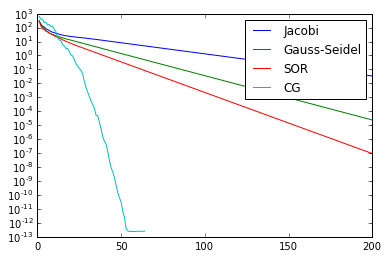
\includegraphics[width=0.5\textwidth]{sor.png}
\caption{Residuals versus iterations}
\end{figure}

We can precondition(\textcolor{red}{or shampoo!}) the conjugate gradient using an incomplete LU decomposition. After preconditioning conjugate gradient, we get
\begin{figure}[H]
\centering
\includegraphics[width=0.5\textwidth]{cg.png}
\caption{Residuals versus iterations before and after preconditioning}
\end{figure}

Here, you can see the plot of number of iterations versus mesh size needed to reach a tolerance of 10e-13 for preconditioned conjugate gradient and 10e-5 for regular CG.
The x axis is the number of sub-intervals. So, if it is n, the system we are solving is $n^2$

\begin{figure}[H]
    \centering
    \begin{subfigure}[b]{0.4\textwidth}
        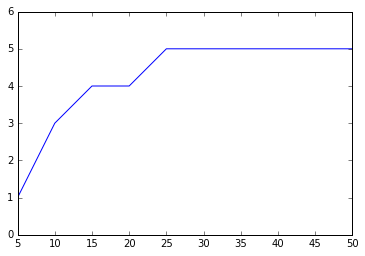
\includegraphics[width=\textwidth]{iter}
        \caption{Preconditioned CG}
        \label{fig:gull}
    \end{subfigure}
    ~ %add desired spacing between images, e. g. ~, \quad, \qquad, \hfill etc. 
      %(or a blank line to force the subfigure onto a new line)
    \begin{subfigure}[b]{0.4\textwidth}
        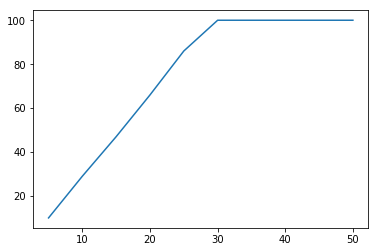
\includegraphics[width=\textwidth]{it2}
        \caption{CG}
        \label{fig:tiger}
    \end{subfigure}
    ~ %add desired spacing between images, e. g. ~, \quad, \qquad, \hfill etc. 
    %(or a blank line to force the subfigure onto a new line)

    \caption{Iterations vs Mesh Size}\label{fig:animals}
\end{figure}
For Conjugate gradient and preconditioned conjugate gradient, the number of iterations needed for a particular accuracy seems to level off more and more as you increase the mesh size. Naturally, the number increases but at a slow rate.
\begin{figure}[H]
    \centering
    \begin{subfigure}[b]{0.3\textwidth}
        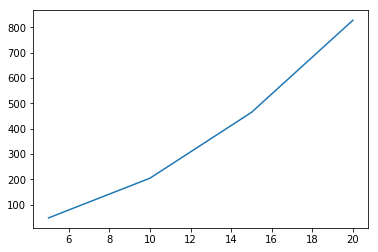
\includegraphics[width=\textwidth]{jit}
        \caption{Jacobi}
        \label{fig:gull}
    \end{subfigure}
    ~ %add desired spacing between images, e. g. ~, \quad, \qquad, \hfill etc. 
      %(or a blank line to force the subfigure onto a new line)
    \begin{subfigure}[b]{0.3\textwidth}
        \includegraphics[width=\textwidth]{gsit}
        \caption{Gauss-Seidel}
        \label{fig:tiger}
    \end{subfigure}
    ~ %add desired spacing between images, e. g. ~, \quad, \qquad, \hfill etc. 
    %(or a blank line to force the subfigure onto a new line)
    \begin{subfigure}[b]{0.3\textwidth}
        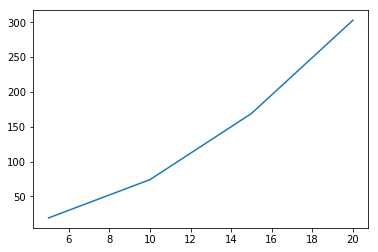
\includegraphics[width=\textwidth]{sorit}
        \caption{SOR}
        \label{fig:tiger}
    \end{subfigure}
    \caption{Iterations vs Mesh Size}\label{fig:animals}
\end{figure}
For the Jacobi, Gauss-Seidel and SOR, the number of iterations needed seem to increase linearly with mesh size.

\begin{lstlisting}[style=myPythonstyle]
import numpy as np
from scipy import sparse
from scipy.sparse import linalg
import matplotlib.pyplot as plt
np.set_printoptions(threshold=np.nan)
np.set_printoptions(precision=5)
import scipy
import scipy.sparse as sp

#  Solves the steady-state heat equation in a square with conductivity
#  c(x,y) = 1 + x^2 + y^2:
#
#     -d/dx( (1+x^2+y^2) du/dx ) - d/dy( (1+x^2+y^2) du/dy ) = f(x),   
#                                                       0 < x,y < 1
#     u(x,0) = u(x,1) = u(0,y) = u(1,y) = 0
#
#  Uses a centered finite difference method.

#  Set up grid.
n = int(input(' Enter number of subintervals in each direction: '));
h = 1/n;
N = (n-1)**2;

# Form block tridiagonal finite difference matrix A and right-hand side 
# vector b.
A = sparse.csr_matrix((N,N));
b = np.ones((N,1));         # Use right-hand side vector of all 1's.

# Loop over grid points in y direction.
for j in range (n-1):
    yj = (j+1)*h;
    yjph = yj+h/2;  yjmh = yj-h/2;

    # Loop over grid points in x direction.
    for i in range(n-1):
        xi = (i+1)*h;
        xiph = xi+h/2;  ximh = xi-h/2;
        aiphj = 1 + xiph**2 + yj**2;
        aimhj = 1 + ximh**2 + yj**2;
        aijph = 1 + xi**2 + yjph**2;
        aijmh = 1 + xi**2 + yjmh**2;
        k = (j)*(n-1) + i;
        A[k,k] = aiphj+aimhj+aijph+aijmh;
        if i > 0: A[k,k-1] = -aimhj; 
        if i < n-2: A[k,k+1] = -aiphj; 
        if j > 0: A[k,k-(n-1)] = -aijmh; 
        if j < n-2: A[k,k+(n-1)] = -aijph; 

A = (1/h**2)*A;   # Remember to multiply A by (1/h^2).
def jacobi_step(u,A,f):
    p = A.diagonal()
    M  = sp.diags(p)
    invM = sp.diags(1/p)
    N = M - A
    G = invM.dot(N)# np.dot(invM,N)
    c = invM.dot(f) #np.dot(invM,f)
    return G.dot(u)+c

def GS_step(u,A,f):
    M  = sp.tril(A)
    #invM = np.diag(1/p)
    N = M - A
    G = sparse.linalg.spsolve(M,N)
    c = sparse.linalg.spsolve(M,f)
    return G.dot(u)+c

def SOR_step(u,A,f,w):
    u_n = GS_step(u,A,f) 
    return (1-w)*u+w*u_n
def res(u,A,f):
    return np.linalg.norm(f-A.dot(u), np.inf)/np.linalg.norm(f, np.inf) 
def steps(A):
    f =np.ones(N)
    u_GS = f
    u_J = f
    u_SOR = f
    resGS = []
    resJ = []
    resSOR = []
    u_CG = f
    resCG = []
    w = 1.36
    for i in range(200):
        u_GS = GS_step(u_GS,A,f)
        resGS = resGS + [res(u_GS,A,f)]
        u_J = jacobi_step(u_J,A,f)
        resJ = resJ + [res(u_J,A,f)]
        u_SOR = SOR_step(u_SOR,A,f,w)
        resSOR = resSOR + [res(u_SOR,A,f)]
        u_CG = scipy.sparse.linalg.cg(A,f,x0=u_CG,maxiter=1)[0]
        resCG = resCG + [res(u_CG,A,f)]
    return resJ,resGS,resSOR,resCG

def green(u):
    global Aw
    global resy
    Aw = Aw + [u]
    resy = resy +[res(u,A,f)]
def precond(A):
    
    w = scipy.sparse.linalg.spilu(A)
    #print(len(w.perm_r))
    Pr = scipy.sparse.csc_matrix((N, N)) 
    Pr[w.perm_r, np.arange(N)] = 1
    Pc = scipy.sparse.csc_matrix((N, N))
    Pc[np.arange(N), w.perm_c] = 1
    L = scipy.sparse.linalg.inv(w.L)
    U = scipy.sparse.linalg.inv(w.U)
    return Pc*U*L*Pr
    
    
def CGsteps(A):
    f =np.ones(N)
    global f,Aw,resy
    
    u_CG = f
    resCG = []
    uw = []
    Aw = []
    resy =[]
    M = precond(A)
    u_CG = scipy.sparse.linalg.cg(A,f,x0=u_CG,maxiter=100,M=M,tol = 1e-5,callback = green)[0]
    return uw,resCG
#a,b,c,d = steps(A)
u_n,resn = CGsteps(A)
print(len(resy))
resy = np.r_[resy,np.zeros(200-len(resy))]
x = np.linspace(1,200,200)
#plt.semilogy(x,a, label='Jacobi')
#plt.semilogy(x,b ,label='Gauss-Seidel')
#plt.semilogy(x,c ,label='SOR')
#plt.semilogy(x,resy ,label='CG')
#plt.semilogy(x,resy2 ,label='Preconditioned CG')
#plt.legend()

# Solve linear system.
#u_comp = sparse.linalg.spsolve(A,b)
\end{lstlisting}

\item 
Suppose a symmetric positive definite matrix $A$ has one thousand eigenvalues
uniformly distributed between $1$ and $10$, and one eigenvalue of $10^4$.
Suppose another symmetric positive definite matrix $B$ has an eigenvalue
of $1$ and has one thousand eigenvalues uniformly distributed between $10^3$
and $10^4$.
Since each matrix has condition number $\kappa = 10^4$, we have seen
that the error at step $k$ of the CG algorithm satisfies
\[
\frac{\| e^{(k)} \|_{A,B}}{\| e^{(0)} \|_{A,B}} \leq 2 \left( \frac{
\sqrt{\kappa} - 1}{\sqrt{\kappa} +1} \right)^k = 2 \left( \frac{99}{101} 
\right)^k .
\]
Give another bound on $\| e^{(k)} \|_A / \| e^{(0)} \|_A$ based
on a polynomial that is a product of a degree $k-1$ Tchebyshev polynomial
on the interval $[1,10]$ and a linear polynomial that is $1$ at the
origin and $0$ at $10^4$.  Give another bound on $\| e^{(k)} \|_B /
\| e^{(0)} \|_B$ based on a polynomial that is a product of a degree $k-1$ 
Tchebyshev polynomial on the interval $[ 10^3 , 10^4]$ and a linear polynomial
that is $1$ at the origin and $0$ at $1$.  For which matrix would you
expect CG to converge more rapidly?  [If you are not sure, you may try
it in Matlab.]

{\bf Solution:}

From 4.51, we know
\[
\frac{\| e^{(k)} \|_{A}}{\| e^{(0)} \|_{A}} \leq \max_j P_k(\lambda_j)
\]

where P is a polynomial of degree at most k such that P(0) =1.
For A, we choose
\[P_k(x) = \frac{T_k(\frac{\lambda_{1000} + \lambda_1-2x}{\lambda_{1000} - \lambda_1})}{T_k(\frac{\lambda_{1000} + \lambda_1}{\lambda_{1000} - \lambda_1})} (1-\frac{x}{10^4})\]
When x is in between 0 and $10^4$,
\[\max P_k(x) \leq \max \frac{T_k(\frac{\lambda_{1000} + \lambda_1-2x}{\lambda_{1000} - \lambda_1})}{T_k(\frac{\lambda_{1000} + \lambda_1}{\lambda_{1000} - \lambda_1})} \max(1-\frac{x}{10^4})\]
\[\leq \max \frac{T_k(\frac{\lambda_{1000} + \lambda_1-2x}{\lambda_{1000} - \lambda_1})}{T_k(\frac{\lambda_{1000} + \lambda_1}{\lambda_{1000} - \lambda_1})}\]
\[\leq 2 \left( \frac{
\sqrt{\kappa} - 1}{\sqrt{\kappa} +1} \right)^k \]
Here, $\kappa = \frac{10}{1}$. So,
\[
\frac{\| e^{(k)} \|_{A}}{\| e^{(0)} \|_{A}} \leq 2(0.5195)^k
\]
For B, we choose
\[P_k(x) = \frac{T_k(\frac{\lambda_{1001} + \lambda_2-2x}{\lambda_{1000} - \lambda_1})}{T_k(\frac{\lambda_{1001} + \lambda_2}{\lambda_{1001} - \lambda_2})} (1-x)\]
When x is in between 0 and $10^4$,
\[\max |P_k(x)| \leq \max |\frac{T_k(\frac{\lambda_{1001} + \lambda_2-2x}{\lambda_{1000} - \lambda_1})}{T_k(\frac{\lambda_{1001} + \lambda_2}{\lambda_{1001} - \lambda_2})}| \max|(1-\frac{x}{10^4})|\]
\[\leq 9999 \max \frac{T_k(\frac{\lambda_{1001} + \lambda_2-2x}{\lambda_{1000} - \lambda_1})}{T_k(\frac{\lambda_{1001} + \lambda_2}{\lambda_{1001} - \lambda_2})}\]
\[\leq 19998 \left( \frac{
\sqrt{\kappa} - 1}{\sqrt{\kappa} +1} \right)^k \]
Here, $\kappa = \frac{10^4}{10^3}$. So,
\[
\frac{\| e^{(k)} \|_{B}}{\| e^{(0)} \|_{B}} \leq 19998(0.5195)^k
\]
I would expect A to converge quicker because it has a lower error bound.
\item
Repeat the experiments on p.~103 of the text, leading to Figures 4.8 and
4.9, but use the Gauss-Seidel method and (unpreconditioned) CG instead of 
Jacobi iteration.  
That is, set up difference equations for the problem
\[
u''(x) = f(x),~~~u(0) = 1 ,~u(1) = 3 ,
\]
where
\[
f(x) = -20 + a \phi'' (x) \cos( \phi (x)) - a ( \phi' (x) )^2 \sin ( \phi (x) ),
\]
where $a = 0.5$ and $\phi (x) = 20 \pi x^3$.  The true solution is
\[
u(x) = 1 + 12 x - 10 x^2 + a \sin ( \phi (x) ) .
\]
Starting with initial guess $u^{(0)}$ with components $1 + 2 x_i$, 
$i=1, \ldots , 255$, run, say, $20$ Gauss-Seidel iterations and then
$20$ CG iterations, plotting the true solution to the linear system 
and the approximate solution, say, at steps 0, 5, 10, and 20, and 
also plotting the error (the difference between true and approximate 
solution).  Print the size of the error (the $L_2$-norm or the $\infty$-norm) 
at these steps too.  Based on your results, would you say that Gauss-Seidel 
and CG would be effective smoothers for a multigrid method?


{\bf Solution:}

The infinity norm is used here. The E stands for error.
\begin{figure}[H]
    \centering
    \begin{subfigure}[b]{0.22\textwidth}
        \includegraphics[width=\textwidth]{gs1}
        \caption{k=1}
        \label{fig:gull}
    \end{subfigure}
    ~ %add desired spacing between images, e. g. ~, \quad, \qquad, \hfill etc. 
      %(or a blank line to force the subfigure onto a new line)
    \begin{subfigure}[b]{0.22\textwidth}
        \includegraphics[width=\textwidth]{GS5}
        \caption{k=5}
        \label{fig:tiger}
    \end{subfigure}
    ~ %add desired spacing between images, e. g. ~, \quad, \qquad, \hfill etc. 
    %(or a blank line to force the subfigure onto a new line)
    \begin{subfigure}[b]{0.22\textwidth}
        \includegraphics[width=\textwidth]{gs15}
        \caption{k=15}
        \label{fig:mouse}
    \end{subfigure}
     \begin{subfigure}[b]{0.22\textwidth}
        \includegraphics[width=\textwidth]{GS20}
        \caption{k=20}
        \label{fig:mouse}
    \end{subfigure}
    \caption{Gauss-Seidel solutions}\label{fig:animals}
\end{figure}
\begin{figure}[H]
    \centering
    \begin{subfigure}[b]{0.22\textwidth}
        \includegraphics[width=\textwidth]{ergs0}
        \caption{k=1 (E=30.41)}
        \label{fig:gull}
    \end{subfigure}
    ~ %add desired spacing between images, e. g. ~, \quad, \qquad, \hfill etc. 
      %(or a blank line to force the subfigure onto a new line)
    \begin{subfigure}[b]{0.22\textwidth}
        \includegraphics[width=\textwidth]{ergs5}
        \caption{k=5 (E=30.25)}
        \label{fig:tiger}
    \end{subfigure}
    ~ %add desired spacing between images, e. g. ~, \quad, \qquad, \hfill etc. 
    %(or a blank line to force the subfigure onto a new line)
    \begin{subfigure}[b]{0.22\textwidth}
        \includegraphics[width=\textwidth]{ergs15}
        \caption{k=15 (E=30.13)}
        \label{fig:mouse}
    \end{subfigure}
     \begin{subfigure}[b]{0.22\textwidth}
        \includegraphics[width=\textwidth]{ergs20}
        \caption{k=20 (E=30.10)}
        \label{fig:mouse}
    \end{subfigure}
    \caption{Gauss-Seidel errors}\label{fig:animals}
\end{figure}


\begin{figure}[H]
    \centering
    \begin{subfigure}[b]{0.22\textwidth}
        \includegraphics[width=\textwidth]{cg0}
        \caption{k=0}
        \label{fig:gull}
    \end{subfigure}
    ~ %add desired spacing between images, e. g. ~, \quad, \qquad, \hfill etc. 
      %(or a blank line to force the subfigure onto a new line)
    \begin{subfigure}[b]{0.22\textwidth}
        \includegraphics[width=\textwidth]{cg5}
        \caption{k=5}
        \label{fig:tiger}
    \end{subfigure}
    ~ %add desired spacing between images, e. g. ~, \quad, \qquad, \hfill etc. 
    %(or a blank line to force the subfigure onto a new line)
    \begin{subfigure}[b]{0.22\textwidth}
        \includegraphics[width=\textwidth]{cg15}
        \caption{k=15}
        \label{fig:mouse}
    \end{subfigure}
     \begin{subfigure}[b]{0.22\textwidth}
        \includegraphics[width=\textwidth]{cg20}
        \caption{k=20}
        \label{fig:mouse}
    \end{subfigure}
    \caption{Conjugate Gradient solutions}\label{fig:animals}
\end{figure}
\begin{figure}[H]
    \centering
    \begin{subfigure}[b]{0.22\textwidth}
        \includegraphics[width=\textwidth]{ercg0}
        \caption{k=1 (E=30.30)}
        \label{fig:gull}
    \end{subfigure}
    ~ %add desired spacing between images, e. g. ~, \quad, \qquad, \hfill etc. 
      %(or a blank line to force the subfigure onto a new line)
    \begin{subfigure}[b]{0.22\textwidth}
        \includegraphics[width=\textwidth]{ercg5}
        \caption{k=5 (E=30.130)}
        \label{fig:tiger}
    \end{subfigure}
    ~ %add desired spacing between images, e. g. ~, \quad, \qquad, \hfill etc. 
    %(or a blank line to force the subfigure onto a new line)
    \begin{subfigure}[b]{0.22\textwidth}
        \includegraphics[width=\textwidth]{ercg15}
        \caption{k=15 (E=29.89)}
        \label{fig:mouse}
    \end{subfigure}
     \begin{subfigure}[b]{0.22\textwidth}
        \includegraphics[width=\textwidth]{ercg20}
        \caption{k=20 (E=29.78)}
        \label{fig:mouse}
    \end{subfigure}
    \caption{Conjugate Gradient errors}\label{fig:animals}
\end{figure}



	\begin{lstlisting}[style=myPythonstyle]
import numpy as np
from scipy import sparse
from scipy.sparse import linalg
import matplotlib.pyplot as plt
np.set_printoptions(threshold=np.nan)
np.set_printoptions(precision=5)
import scipy
import scipy.sparse as sp

def tridiag(a, b, c, k1=-1, k2=0, k3=1):
    return np.diag(a, k1) + np.diag(b, k2) + np.diag(c, k3)
N = 255
h = 1/(N+1)
a = np.ones(N)
b = np.ones(N-1)
A = ((N+1)**2)*tridiag(b,-2*a,b)
def u_init(x):
    return 1+2*x
xout = np.linspace(0,1,N+2)
x = xout[1:-1]
def u_true(x):
    return 1+12*x-10*x**2+0.5*np.sin(p(x))
def p(x):
    return 20*np.pi*x**3
def make_f(x):
    return -20 + 0.5* 120*np.pi*x*np.cos(p(x))-0.5*((60*np.pi*x**2)**2)*np.sin(p(x))
def GS_step(u,A,f):
    M  = np.tril(A)
    #invM = np.diag(1/p)
    N = M - A
    G = scipy.linalg.solve(M,N)
    c = scipy.linalg.solve(M,f)
    return np.dot(G,u)+c
def make_b(f):
    b = f
    b[0] = b[0] - (N+1)**2
    b[-1] = b[-1]-3*(N+1)**2
    return b
f = make_f(x)
b = make_b(f)
#u = np.linalg.solve(A,b)
def res(u,A,f):
    return np.linalg.norm(f-A.dot(u), np.inf)/np.linalg.norm(f, np.inf) 
def steps(A,b):
    u_n = u_init(x)
    u_t = u_true(x)
    resn = []
    u_nw=[]
    for i in range(20):
        u_n = GS_step(u_n,A,b)
        u_nw = u_nw +[u_n]
        resn = resn + [[abs(u_n-u_t)]]
    return u_nw,resn
#plt.plot(u)
u,resn = steps(A,b)
def green(u):
    global Aw
    global resy
    Aw = Aw + [u]
    resy = resy +[[abs(u-u_t)]]
    
def CGsteps(A,b):
    f =np.ones(N)
    global f,Aw,resy, u_t
    
    u_i = u_init(x)
    resCG = []
    u_t = u_true(x)
    
    uw = []
    Aw = [u_i]
    resy =[]
    u_CG = scipy.sparse.linalg.cg(A,b,x0=u_i,maxiter=20, callback = green)[0]
    return uw,resCG
uw,resw = CGsteps(A,b)
#plt.semilogy(resn)
\end{lstlisting}
\end{enumerate}

\end{document}
